\chapter{Time Delay Compensation and Predictive Display}
\label{ch_7:PDsply}
In the last chapter it was shown using simulation results that time delay between the remote and local station leads the system towards instability. In this chapter we first present predictive model controller for time delayed teleoperation. We then highlight the issues of time delay on human performance. We then present our  RGB-Depth sensor based  predictive display implemented in our system  to alleviate the problem of time delay in visual feedback.

\section {Model Based Time Delay Compensation}
As shown in the last chapter, simulation of time delays system with pure pursuit model for human controller in stability starts with as the delay in feedback i.e input delay to the human model increase. In paper by Ollero \cite{ollero1995stability} stability of pure pursuit with input delay was presented. The details of which is presented in Appendix \ref{appendix_b}.   In view of the above theoretical analysis and the simulation results presented in the last chapter its required to design  a stabilizing controller to take care of large delays i.e 0.8 sec. One such design based on model based predictive control is presented next.

 \begin{figure}
 	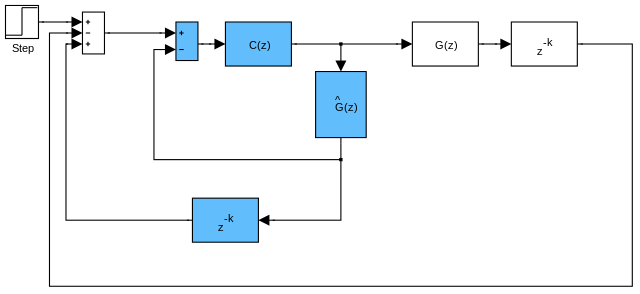
\includegraphics[width=\linewidth]{Chapter7/fig/Smith_predictor}
 	\caption{Smith Predictor}
 	\label{fig:Smith}
 \end{figure}
 
 One of the earliest predictor based controller for Linear system with time delay  was proposed by Smith \cite{smith1959controller} called the Smith Predictor or Smith Controller. The schematic of the smith controller is shown in figure \ref{fig:Smith}. There are two loops the inner and the outer loop. Where $G(z)$ is the plant, $C(z)$ is the stabilizing controller  for plant with out delay, $\hat{G}(z)$ is the model of the plant.  As can be seen from the figure \ref{fig:Smith} that during the period (k time unit ) when the feedback (output) is not available the model of the plant is used to predict the actual plant behaviour and generate the control signal accordingly. 
 
 In our case the plant is a mobile robot. The block digram shown in Figure \ref{fig:blockdigTimeDelay} depicts the architecture of the time delay system applicable to the current system. The teleoperation  over wireless network for our system   resulted in a delay of $T_1= 500~ms$, or update frequency of 2Hz,  for the video feedback from robot camera. This is due to the large amount of data being transmitted. The Figure \ref{fig:delayphoto} shows the measured delay in video link. The frequency of odometric and control  data exchange between the two stations was at the rate of 20Hz, ie a delay $T_2=50ms$. This  loop runs was independent of the video feedback link.  It may be noted that $T_2<<T_1$ for this system.
 \begin{figure}[ht]
 	\centering
 	\begin{minipage}{0.45\textwidth}
 		\centering
 		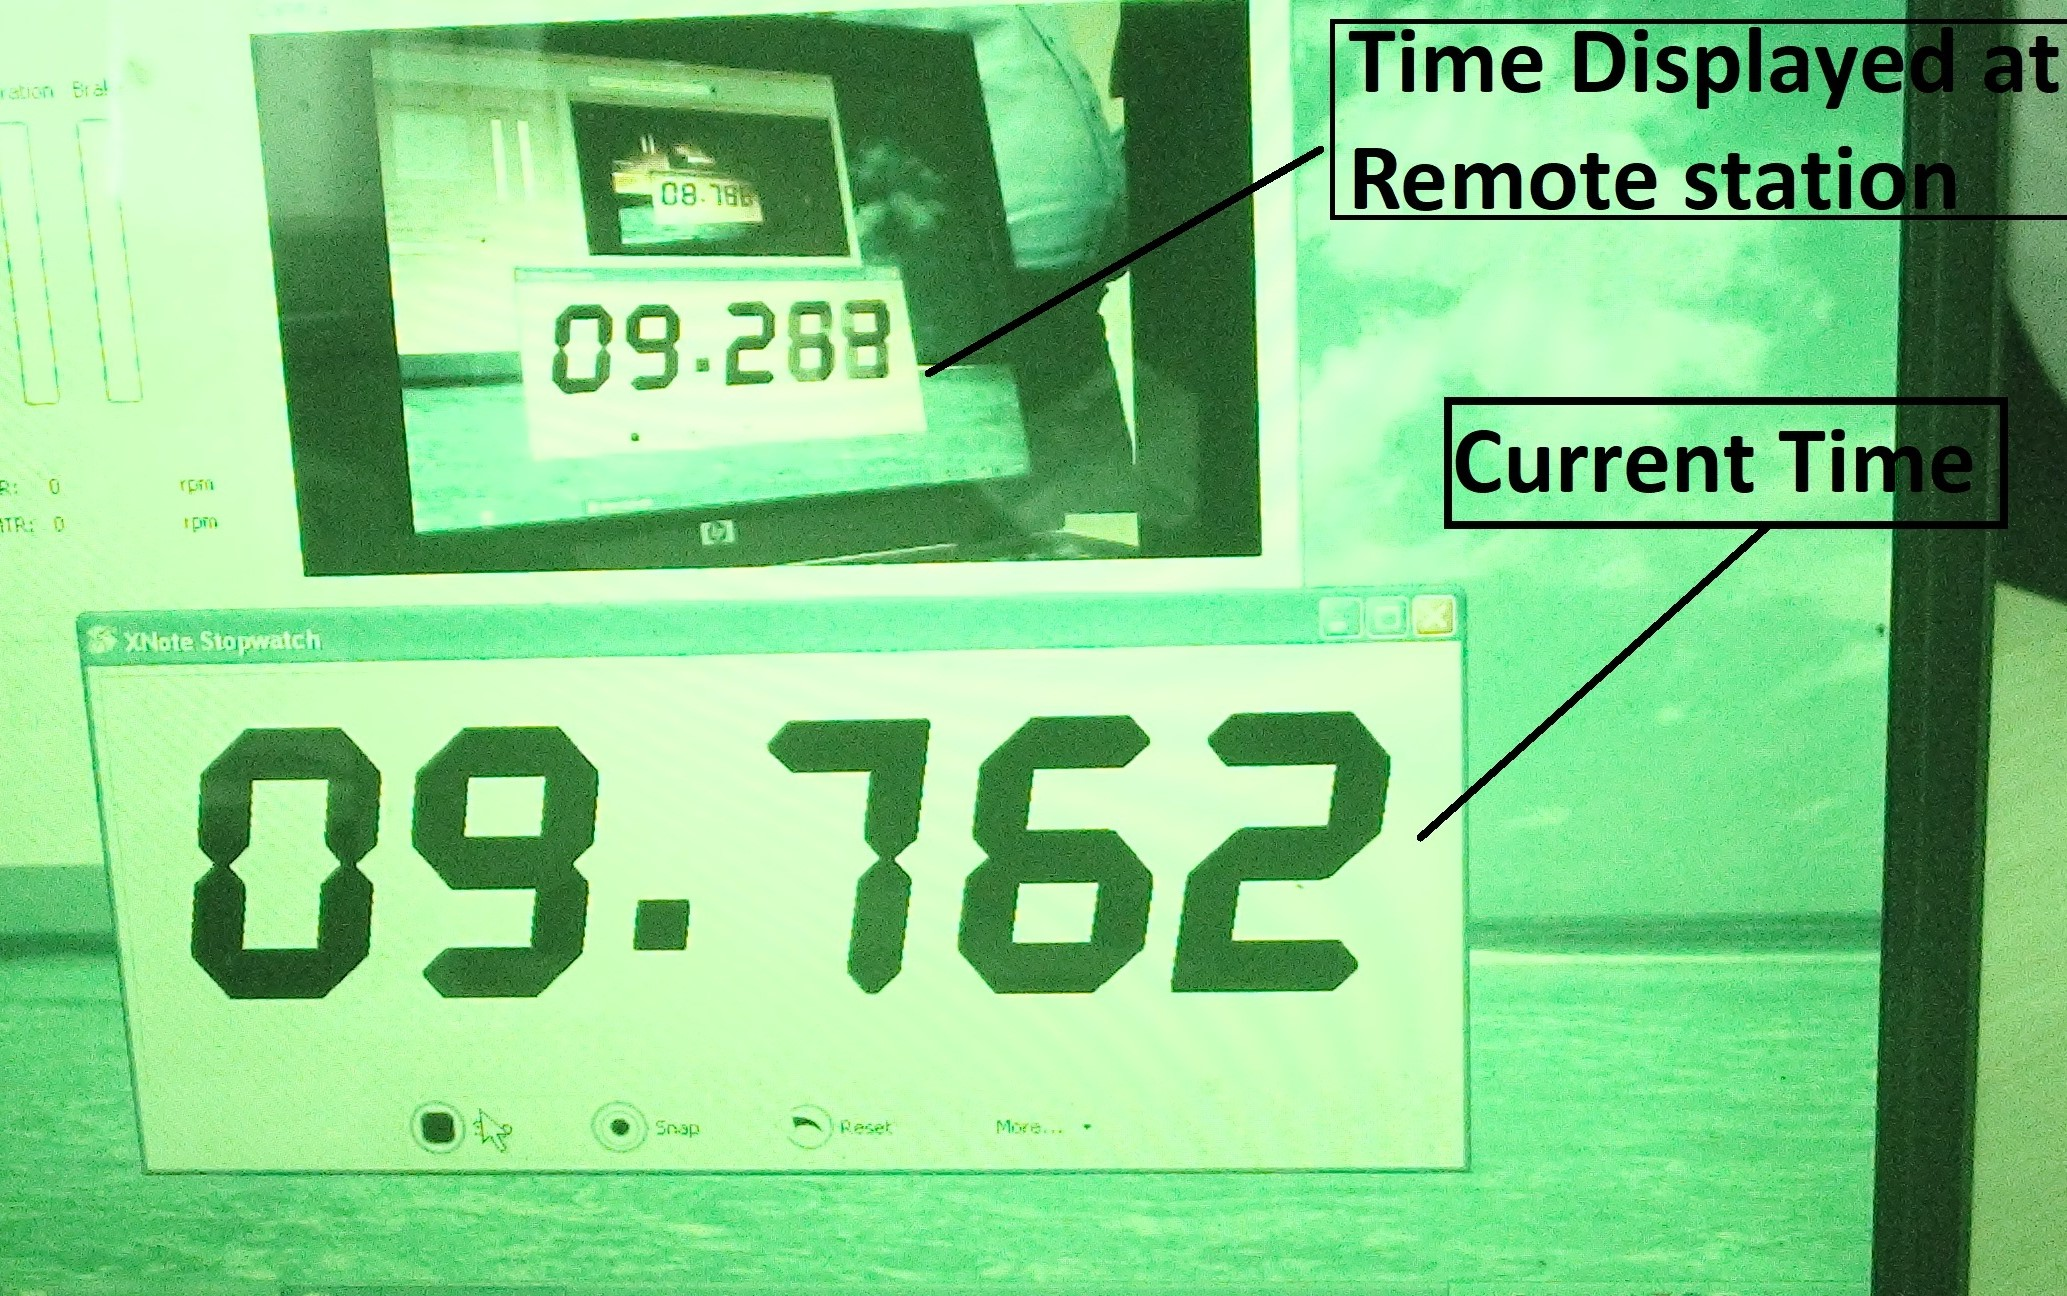
\includegraphics[width=\linewidth,keepaspectratio]{Chapter7/fig/delayMeasureNew}
 		\captionof{figure}{Delay measurment}
 		\label{fig:delayphoto}
 	\end{minipage}%
 	\begin{minipage}{0.55\textwidth}
 		\centering
 		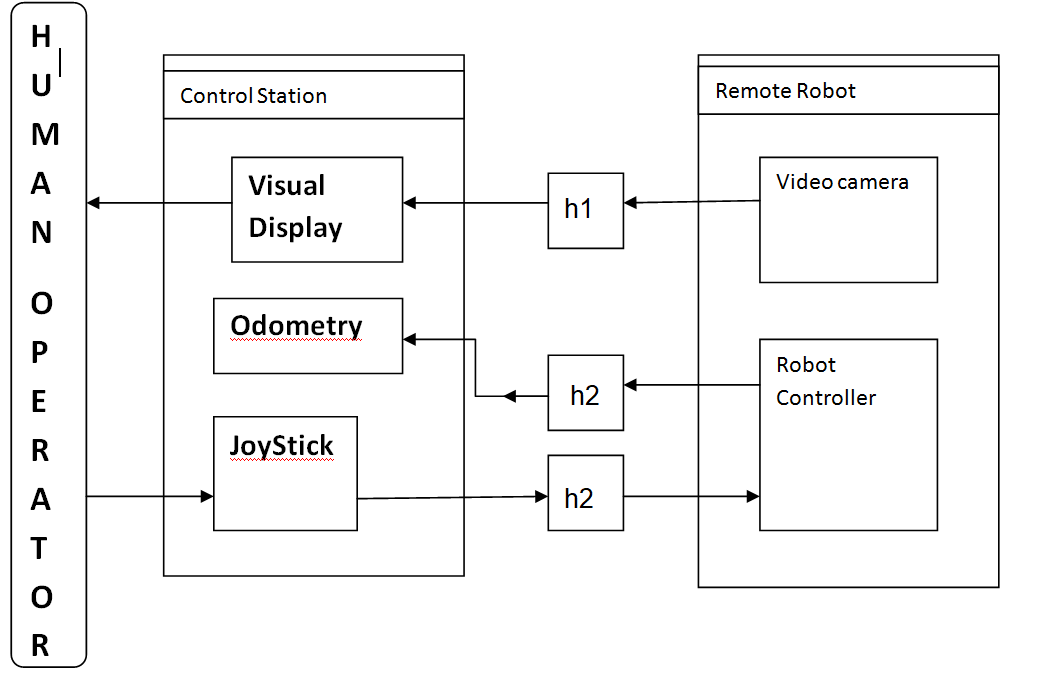
\includegraphics[width=.9\linewidth,keepaspectratio]{Chapter7/fig/BlockTimeDelay}
 		\captionof{figure}{Block digram of \\time delay system}
 		\label{fig:blockdigTimeDelay}
 	\end{minipage}
 \end{figure} 

%This was possible because  A new pose was predicted based on the odometric data and fed to the "human operator model" for the intermediate control action.
\subsection{Proposed Controller}
The proposed control strategy to mitigate the effect of time delay is to predict the current position based on the dynamic model of the mobile robot from the last known position from the delayed video image.  As shown in Figure \ref{fig:SmithRobot} let us assume that we are at time $t+\delta$, but the latest pose  data of the robot available is that of at time $t$. We predict the present pose i.e at time $t+\delta$ based on the dynamic model  of the robot derived in Chapter \ref{c4_Dynamics}, Equation \ref{CE}, and presented here again for convenience. 
\begin{equation}
\label{CE2}
\quad I(\theta)\ddot{\theta}=C(\theta,\dot{\theta})\dot{\theta}+\tau
\end{equation}
It may be noted that the dynamic model uses torque $\tau$ as it input. Where as the local station which uses, pure pursuit for sumulation of  human action,   generates Linear  $v$ and Angular $\dot\theta$  velocities of the robot as shown in Figure \ref{fig:SimBlock}. This is taken care by first converting $V \equiv\dot o_3$ and $\dot\theta\equiv\omega_3$ to rear wheel velocities using Equations \ref{omegaPlat} and \ref{velPlat}. The rear wheel velocities  are then used in PI controller given Chapter \ref{c5_Control} of the rear wheel motors to generate the $\tau$ for Equation \ref{CE2}.

This predicted position is given to the pure pursuit algorithm to generate required control outputs for the remote robot. In the simulation it is assumed that this control inputs reaches the remote robot instantaneously, as $T_1>> T_2$. As discuss in the Chapter \ref{c6_simulation}   Kinematic model given by Equation \ref{eqn:KinematicModelOfRobot} is used to simulate remote robot.
 \begin{figure}
	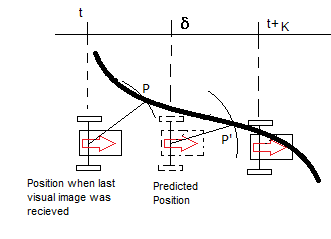
\includegraphics[width=1.2\linewidth]{Chapter7/fig/robotPredictPos}
	\caption{Smith predictor applied to mobile robot}
	\label{fig:SmithRobot}
\end{figure}
 \begin{figure}
	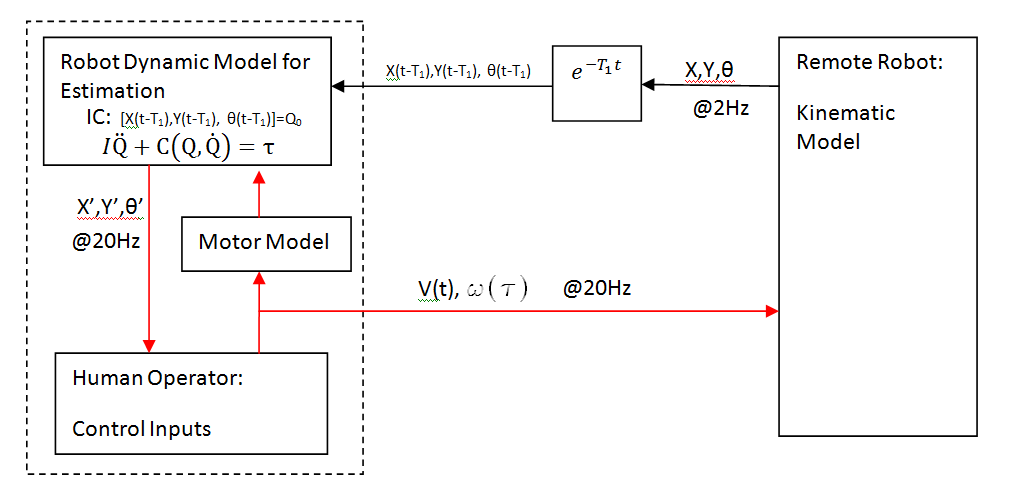
\includegraphics[width=\linewidth]{Chapter7/fig/Sumilation_BlkDgm}
	\caption{Simulation block Digram}
	\label{fig:SimBlock}
\end{figure}
\subsection{Simulation algorithm and  results} 
The simulation scheme is  shown in block digram shown in Figure \ref{fig:SimBlock}. The algorithm  is explained  below.

\begin{algorithmic}[1]
	\State Convert the path from global coordinate system (CS) to Robots Local Coordinate System based current pose  $(x,y,\theta)$ of robot.
	\State With a given look ahead distance (l) search for a goal point on the path.
	\State Determine the turning radius (r) using Equation 6.5 
	\State Calculate $\omega$ using turning radius (r) and given Linear Velocity $V$
	\State Command Robot $\omega$ and  $V$
	\If  {new pose of robot available from remote station}
		\State Update robot pose $(x,y,\theta)$
	\Else
		\State Calculate the predicted pose of the robot  based on commanded given in Step 4, using dynamic model of robot given in Equation \ref{CE2}.
		\State Update robot pose $(x,y,\theta)$ 
	\EndIf
	\State\textbf{ Goto} Step 1
\end{algorithmic}	
 Simulation was carried using Matlab. Differential equation solver \textit{"Ode24"} was used to solve equation \ref{eqn:KinematicModelOfRobot} and \ref{CE2}.  The desired path  was a circle of radius 5m centred at origin of the global coordinate system. The human action was modelled with look ahead distance $l$, of 0.5m and linear velocity $V$, of 0.5m/s. The initial position of the robot was (4.5,0.0).
 
 The  robot's motion  under feedback delay of 0.5 and 0.8 sec i.e.  $T_1=0.5sec$ and $T_1=0.8sec$,  is shown in  Figures \ref{fig:PreDelay500plot} and \ref{fig:PreDelay800plot} respectively.   It is seen that oscillation are no more visible at 0.5sec delay and with the delay of  0.8 sec. The system shows no instability. 

 \begin{figure}[h]
 	 \begin{minipage}[T]{0.5\linewidth}
 	 	\centering
 		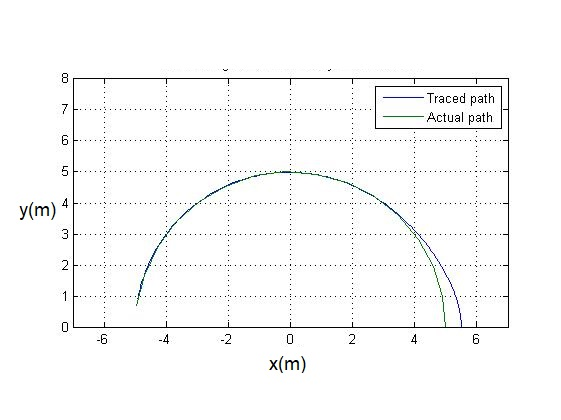
\includegraphics[width=\linewidth,keepaspectratio]{Chapter7/fig/withPrediction05dely}
 		\captionof{figure}{Time delay $T_1=.5sec$ and $T_2=0$ }
 		\label{fig:PreDelay500plot} ...
 	\end{minipage}
 \hfill
 	\begin{minipage}[T]{0.5\linewidth}
 		\centering
		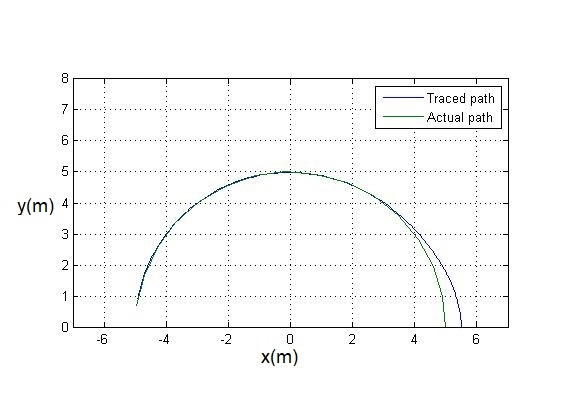
\includegraphics[width=\linewidth,keepaspectratio]{Chapter7/fig/withPrediction08delay}
		\captionof{figure}{Time delay $T_1=.8sec$ and $T_2=0$ }
		\label{fig:PreDelay800plot} 
 	\end{minipage}
 \end{figure} 


The above result shows that model based prediction of robot pose helps in removing the instability of the system. In  actual teleoperation, the operator's control actions are based on the visual display available to him.  The delay in visual feedback results in inefficient operator performance, as the operator tends to adopts a wait and watch policy to see the affect of his control action. In the next section, we present  an implementation and adaptation  of above discussed \textit{model based prediction method}  for  visual display feedback.   
  
\section{Predictive Display}
As indicated in chapter on literature survey,  the delay of visual feedback leads to inefficient and unstable performance of teleoperation system. There are two major methods to over come this time delay induced problem in teleoperation. One is to use \textit{supervisory control} and the other is \textit{predictive display}. We adopt the second methodology ie, the Predictive Display, in our teleoperation architecture. This is because it is more intuitive to human operator, and the onboard controller  required on the mobile robot is very much simplified.  

  
Predictive display has been defined as using the computer for extrapolating the display forward in time \cite{sheridan}. In this a local model of the remote scene is used to predict and render the remote scene in response to operator command. It replaces the delayed video feedback with extrapolated synthesised  image of the remote environment. This enables the operator to perform the task normally. Predictive display has been implemented in the past using different sensor such as monocular camera fixed on the wall, camera mounted on the robot arm, fusion of Lidar scanner and RGB camera, etc as has been discussed in literature survey. 
Our approach is to use low cost  Kinect Sensor from Microsoft Inc. to generate 3-D model of the remote environment and use kinematic model of the mobile robot to predict the motion of actual robot in this 3-D model to generate delay free estimated image of the remote environment to the operator.

\subsection{Depth Sensor Kinect}
\begin{figure}
	\includegraphics[width=\linewidth,keepaspectratio]{Chapter7/fig/kinect}
	\caption{Kinect Sensor from Microsoft}	\label{fig:Kinect}
\end{figure}
Kinect sensor from microsoft is shown in Figure \ref{fig:Kinect}. The hardware contains a normal RGB camera, a depth sensor and a four-microphone array, which are able to provide  RGB images,  depth signals, and audio signals simultaneously. The depth sensor comprises the Infra Red (IR) projector and the IR camera. The IR projector casts an IR speckle dot of known  pattern into the 3-D scene while the IR camera captures the reflected IR speckles. To determine the depth, triangulation method.  Kinect is therefore an instance of a structured light depth sensor. More details concerning the structured light 3-D imaging technology can be found in \cite{geng2011structured}. 

The \textit{RGB camera}  delivers three basic colour components of the video. The camera operates at 30 Hz, and can offer images at $640\times480$ pixels with 8-bit per channel. The  \textit{3-D Depth Sensor} create a depth map, which provides the distance information between an object and the camera. The sensor has a practical ranging limit of 0.8m-3.5m distance, and outputs video at a frame rate of 30 frames with the resolution of 640 x 480 pixels. The angular field of view is $57^o$ horizontally and $43^o$ vertically.
Number of different open source software libraries are available  which includes OpenNI \cite{openni} , Microsoft Kinect SDK  \cite{mssdk} and OpenKinect \cite{freenect} to access the Kinect sensor data. We used OpenNi as it is compatable with RTabMap an Open Source Software used for reconstruction of 3-D point cloud model of remote environment. 

\subsection{Onboard Data processing and transmission}
In our teleoperation structure the Kinect sensor mounted on the mobile robot is connected with the onboard Raspberry Pi single board computer with limited processing power. The onboard controller uses OpenNi library to interface with the kinect hardware.  The Kinect sensor has two separate cameras. The transformation between the camera centres are known and provided the manufacturer. It therefore generates two stream the colour and depth data stream. It is possible to send the two raw data streams over the network combine without any processing at the robot side. This  puts less stresses on the onboard compute but requires high communication bandwidth. The other option is to stream \textit{ registered depth} data over the network. This requires less bandwidth as each pixel has both the colour and depth value associated with it when it is transmitted. Depth Registration requires minimal computing power. Where the known transformation between the two cameras is used to align the depth pixel and the colour pixel so that they correspond to the same point of the 3-D scene. This is referred to as \textit{depth registration} or \textit{image registration} in literature, The word "depth" in the   \textit{depth registration} indicates  that the final image data is with respect to  the depth camera frame. We adopt the second method in our architecture. Where the robot transmits registered depth data, i.e. the RGB and the Depth (RGB-D) value associated with each pixel to the control station over network. 


\begin{figure}
	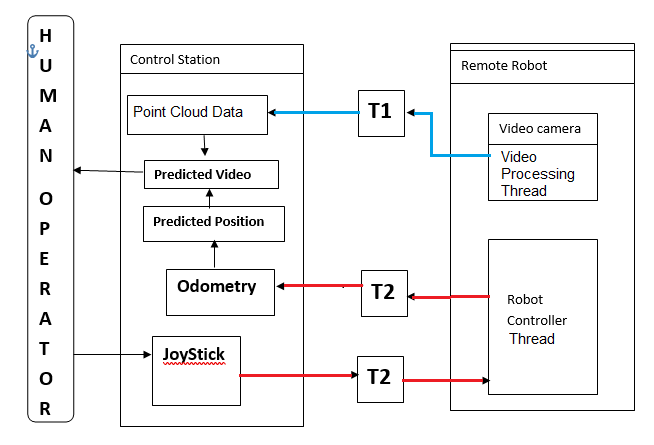
\includegraphics[width=1.2\linewidth,keepaspectratio]{Chapter7/fig/PredictorBlockDig}
	\caption{Predictive display architecture}	\label{fig:PDBLock}
\end{figure}

\subsection{3-D Reconstruction at operator station}
The registered depth data received at the operator station is processed using the RTabMap library \cite{rtabmap} and 3 Pint Cloud data is generated. The details of the working of RTabMap can be found in \cite{labbertab} and \cite{labbe2013appearance}.  Point cloud map is a set of points in 3-D space derived using the camera model and the depth data associated with each pixel of the depth registered data sent from the mobile robot. Each new frame that arrives is added to the current data set after proper transformation. The transformation between two frames of data is created by matching the common feature in the two frame. The RTabMap library thus outputs a set of 3-D point along with there RGB color. The coordinates of the points are always  w.r.t to camera coordinate frame. It may be noted that the registered depth image that has arrived is $T_1$ unit of time delayed. So the local station always has a 3-D map w.r.t to the robot at $(t-T_1)$ sec.
 

\subsection{Remote scene extrapolation} 
The visual data present in the current frame is the view that the robot has seen $T_1$ second earlier, let this data be denoted by $P(t-T_1)=Set\{P_i\}$. This point $P_i$, has associated with it coordinate ${Px_i,Py_i,Pz_i}$ and color data $c_i$. In order to predict the current scene that the robot might be seeing we need to estimate the current position of the robot. The teleoperation architecture shown in Figure \ref{fig:PDBLock} is used in our system to accomplish this. As has been stated earlier that the delay $T_2$ in exchange of command data and the wheel velocity data from the robot to the operator station is 20ms, shown in Figure \ref{fig:PDBLock} by red line. It may thus be assumed that the using the odometric Equation \ref{eqn:odo1},~\ref{eqn:odo2} and \ref{eqn:odo3}, the current position of the robot is always know to the operator station. This is performed by Odometric Block in Figure \ref{fig:PDBLock} by calculating Equations \ref{eqn:odo1},~\ref{eqn:odo2} and \ref{eqn:odo3} from time $t-T_2$ to $t$, with \[x(i=0)=0,~y(i=0)=0 ,~ \beta(i=0)=0\] and  \[ i=0 \text{ to } n;  \quad n=T_1/T_2\] 

Let the predicted position of the robot at time $t$ be given by 
\[(x(i),~y(i) ,~ \beta(i))\rightarrow(x_v(t),y_v(t),\beta_v(t))^T\]
This is basically the amount by which the robot has moved after the last video frame had arrived. Next the transformation matrix, $T^c_r$ between the Vehicle coordinate at point $O_r$ in Figure \ref{fig:KenVec} and the camera frame is used to calculate the change in pose of the camera. Since the pints $P_i$ are in th camera frame there current coordinates ${P'x_i,P'y_i,P'z_i}$is arrived at by using 
\begin{eqnarray}
\begin{pmatrix}
P'x_i \\ P'y_i \\P'z_i
\end{pmatrix}=T^c_r
\begin{pmatrix}
Px_i\\Py_i\\Pz_i
\end{pmatrix}
\end{eqnarray}

This new location of the points are now projected to the screen of the local operator. Thus giving him the estimated current view from the robot. 
 \begin{figure}[ht]
	\begin{minipage}{.5\textwidth}
		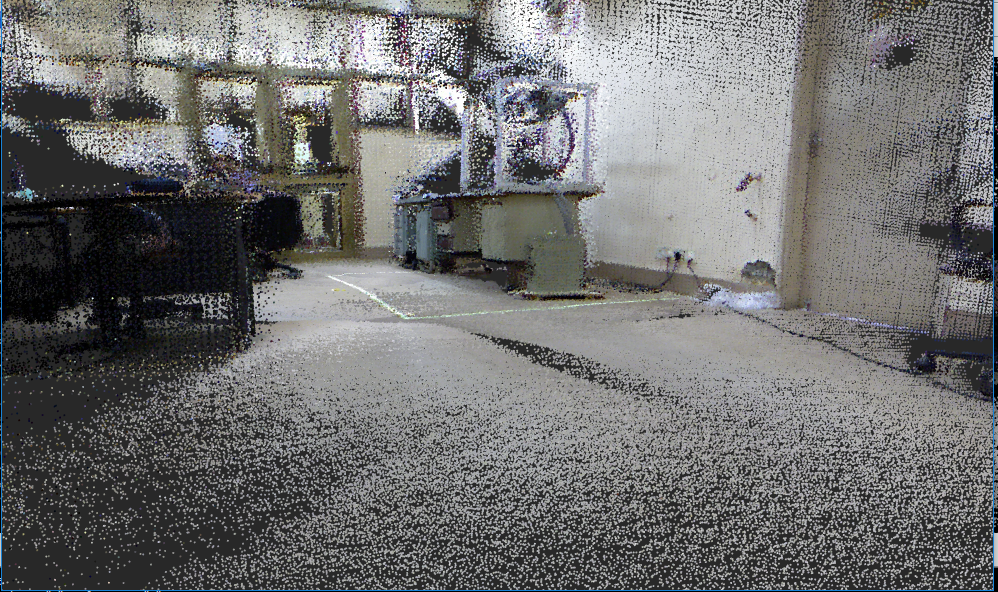
\includegraphics[height=4cm,keepaspectratio]{Chapter7/fig/pcdT}
		\captionof{figure}{PCD at time T }
		\label{fig:pcdt} 
	\end{minipage} 
	\begin{minipage}{.5\textwidth}
		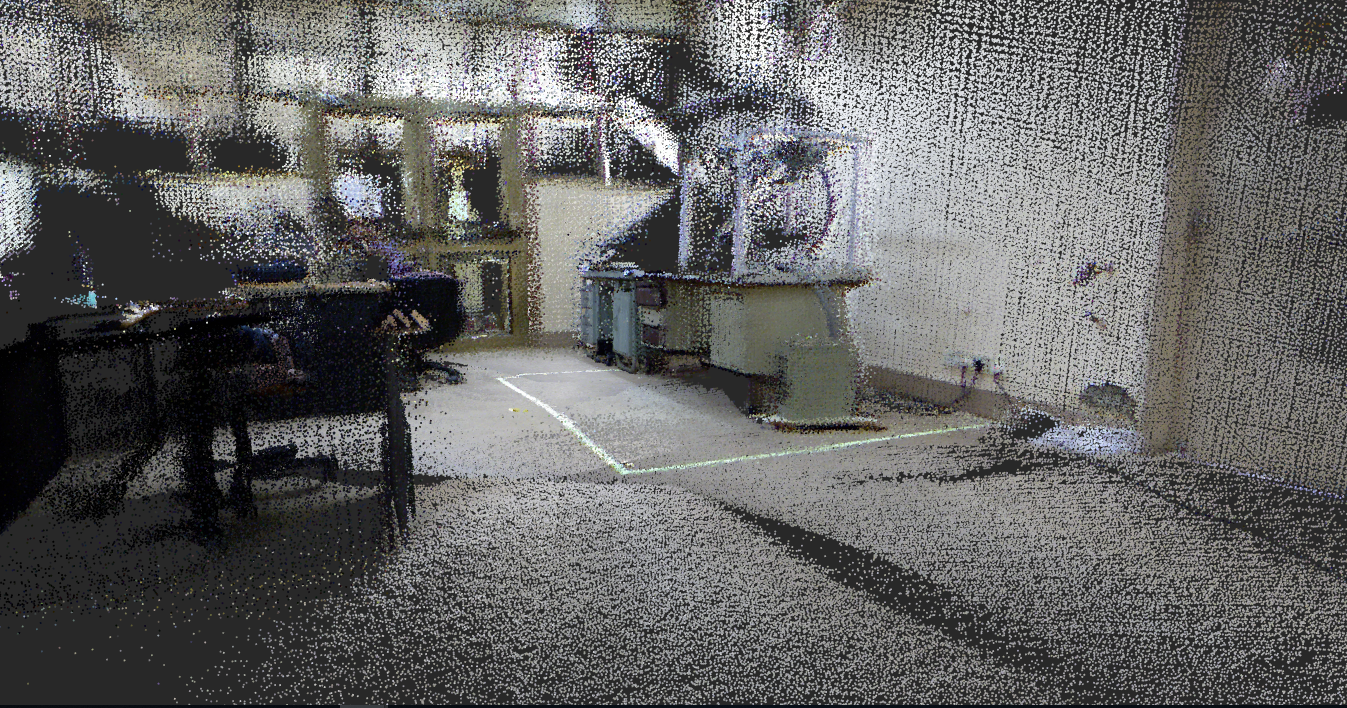
\includegraphics[height=4cm,,keepaspectratio]{Chapter7/fig/pcdT_p}
		\captionof{figure}{Predicted Scene}
		\label{fig:pcdP} 
	\end{minipage}
\end{figure}


The view available at the operator station at time $t$ is shown in Figure \ref{fig:pcdt} which $T_1$ sec old. Based on this old data the predicted scene is shown in Figure \ref{fig:pcdP}.  The operator is sees  Figure \ref{fig:pcdP} instead of Figure \ref{fig:pcdt}.

\section{Result and conclusion}
With this predictive display model the operator was able to move the robot with out wait and see stratagey adopted earlier. 

\section{Summary}
In this chapter we discussed the model based predictive control for control of mobile robot over time delayed network. The stability of the control was verified using simulation. This model was then adopted for visual feedback teleoperation. Were the kinect sensor was used to generate the 3-D model of the remote environment in real time. The estimated position of robot using the odometry was used to project a synthesised image of the 3-D model of the remote environment, from the estimated location to the operator. 
